\subsection{General Terminology and Notation}

Continuous random variables take values on some interval of real numbers. We have $P(X = x) = 0$ for each $x$, because $P(X = a) = \displaystyle \int_{a}^{a} f(x) \, dx = 0$. 

We use the cumulative distribution function $F(x)$ and the probability density function $f(x)$ to describe a continuous random variable.

\begin{definition}[\textbf{Cumulative Distribution Function (c.d.f.)}]
    \phantom{}
    \[F(x) = P(X \leq x).\]
\end{definition}

\begin{theorem}[\textbf{Properties of a c.d.f.}]
    \phantom{}\
    \begin{enumerate}
        \item $F(x)$ is defined $\forall x \in \R$.
        \item $F(x)$ is a non-decreasing function of $x$.
        \item $\dis \lim_{x \to -\infty} F(x) = 0$ and $\dis \lim_{x \to \infty} F(x) = 1$.
        \item  $P(a \leq X \leq b) = F(b) - F(a)$.
    \end{enumerate}
\end{theorem}

\begin{note}
    Since $P(X = x) = 0$ for each $x$, we have \vspace{-3mm}
    \[P(a < X < b) = P(a \leq X \leq b) = P(a \leq X < b) = P(a < X \leq b) = F(b) - F(a).\]
\end{note}

\begin{definition}[\textbf{Probability Density Function (p.d.f.)}]
    \phantom{}\\
    The \textbf{probability density function} $f(x)$ for a continous random variable $X$
    is the derivative \[f(x) = \frac{\dd{F(x)}}{\dd{x}},\]
    where $F(x)$ is the cumulative distribution function for $X$.
\end{definition}

\begin{note}
    From the way in which $X$ was generated that $f(x)$ represents the \textbf{relative likelihood} of (small intervals around) different $x$-values (outcomes).
\end{note}

\pagebreak


\begin{theorem}[\textbf{Properties of a p.d.f.}]
    \phantom{}\\
    Assume that $f(x)$ is a continuous function of $x$ at  all points for which $0 < F(x) < 1$.
\begin{enumerate}
    \item $\dis P(a \leq X \leq b) = F(b) - F(a) = \int_{a}^{b} f(x) \, dx$. \vspace{1mm}
    \item $f(x) \geq 0$ (since $F(x)$ is non-decreasing, so its derivative should be non-negative). \vspace{1mm}
    \item $\displaystyle \int_{-\infty}^{\infty} f(x) \, dx = \displaystyle \int_{\text{all $x$}} f(x) \, dx = 1$.
    \item $F(x) = \displaystyle \int_{-\infty}^{x} f(u) \, du$ (this is property 1 with $a = -\infty$). \\
\end{enumerate}
\end{theorem}

\begin{definition}[\textbf{Quantiles and Percentiles}]
    \phantom{}\\
    Suppose $X$ is a continuous random variable with cumulative distribution function $F(x).$
    The $p$th quantile of $X$ (or of the distribution) is the value $q(p)$, \st $P\left[X \leq q(p)\right] = p.$    \\
    The value $q(p)$ is also called the $100$th percentile of the distribution. If $p = 0.5$, then
    $m = q(0.5)$ is called the median of $X$ or the median of the distribution.
\end{definition}

\begin{remark}
    The \textbf{Median} is the value $m$ such that
    \[
        F(m) = \displaystyle \int_{-\infty}^{m} f(x) \, dx = 0.5 = \displaystyle \int_{m}^{\infty} f(x) \, dx, \text{ which is the 50th percentile.}
    \]
\end{remark}

\begin{example}
    Let
    \[
        F(x) = 
        \begin{cases} 
        0 & \text{for } x \leq 0 \\
        \frac{x}{4} & \text{for } 0 < x \leq 4 \\
        1 & \text{for } x > 4 
        \end{cases}
    \]
    \begin{enumerate}[label=(\alph*)]
        \item Solve for $f(x)$. \\
        \textbf{Solution:} $f(x) = \frac{\dd}{\dd{x}} \left( F(x) \right) = \frac{\dd}{\dd{x}} \left( \frac{x}{4} \right) = \frac{1}{4}$ for $0 < x \leq 4$. Note that outside this interval $f(x)$ is defined to be 0.
        \item Solve for the 90th percentile, i.e. solve for the value of $x$ \st the area under the curve to its left is 0.9. \\
        \textbf{Solution:} Note that the $f(x) = \frac{1}{4}$ is a constant function. \\
        We need to solve for $x$: $F(x) = P(X \leq x) = 0.9$. So, $\frac{1}{4} x = 0.9 \implies x = 3.6$.
    \end{enumerate}
\end{example}

\pagebreak

\begin{example}
    Let $X$ be a continuous random variable with p.d.f.
    \[
        f(x) = 
        \begin{cases} 
        c(4x - 2x^2) & \text{for } 0 < x < 2 \\
        0 & \text{otherwise}
        \end{cases}
    \]
    Find
    \begin{enumerate}[label=(\alph*)]
        \item the constant $c$.
        \item $F(x)$.
        \item $P(X > 1)$.
    \end{enumerate}

    \textbf{Solution:} 
    \begin{enumerate}[label=(\alph*)]
        \item 
        \begin{align*}
            \displaystyle \int_{-\infty}^{\infty} f(x) \, dx &= 1 \\
            \displaystyle \int_{0}^{2} c(4x - 2x^2) \, dx &= 1 \\
            c \left[ 2x^2 - \frac{2x^3}{3} \right]_0^2 &= 1 \\
            &\vdots \\
            c &= \frac{3}{8}
        \end{align*}
        \item $F(X) = P(X \leq x) = \displaystyle \int_{-\infty}^{x} f(u) \, du = \displaystyle \int_{0}^{x} \frac{3}{8} (4u - 2u^2) \, du = \frac{3}{8} \left[ 2u^2 - \frac{2u^3}{3} \right]_0^2 = \frac{3}{8} \left( 2x^2 - \frac{2x^3}{3} \right)$.
        
        Therefore, we have 
        \[
            F(x) = 
            \begin{cases} 
            0 & x \leq 0 \\
            \frac{3}{8} \left( 2x^2 - \frac{2x^3}{3} \right) & 0 < x < 2 \\
            1 & x \geq 2
            \end{cases}.
        \]
        \item $P(X > 1) = \displaystyle \int_{1}^{\infty} f(x) \, dx = \displaystyle \int_{1}^{2} f(x) \, dx = \cdots = 0.5$.
        
        OR \\
        $P(X > 1) = 1 - P(X \leq 1) = 1 - F(1) = \cdots = 0.5$.
    \end{enumerate}
\end{example}

\pagebreak

\textbf{Defined Variables or Change of Variables:}  \\
Suppose we know the p.d.f. or c.d.f. for a continous random variable $X$, we sometimes want to find
the p.d.f. or c.d.f. for some other random variable $Y$, a function of $X$. The procedure is summarized below.
\begin{enumerate}
    \item Write the c.d.f. of $Y$ as a function of $X$.
    \item Use $F_X(x)$ to find $F_Y(x)$. Then if you want the p.d.f. $f_Y(y)$, you can differentiate $F_Y(x)$.
    \item Find the range of values of $y$.
\end{enumerate}

\begin{example}
    $X$ is a continuous random variable having
    \[
        f(x) = \frac{1}{4} \text{ for $0 < x \leq 4$} \quad \text{and} \quad F(x) = \frac{x}{4} \text{ for $0 < x \leq 4$}.
    \]
    Let $Y = \frac{1}{X}$. Find the p.d.f. of $Y$.


    \textbf{Solution:} \\
    Step 1: \vspace{-3mm}
    \begin{align*}
        F_Y(y) = P(Y\leq y) &= P(\frac{1}{X} \leq y) \\
        &= P(X \geq \frac{1}{y}) \\
        &= 1 - P(X \leq \frac{1}{y}) \\
        &= 1 - F_X(\frac{1}{y})
    \end{align*}

    Step 2: 
    \[
        F_Y(y) = 1 - F_X(\frac{1}{y}) = 1 - \frac{\frac{1}{y}}{4} = 1 - \frac{1}{4y}.
    \]
    We can differentiate $F_Y(y)$ to obtain $f_Y(y)$. 
    \[
        f_Y(y) = \frac{\dd}{\dd{y}} \left( 1 - \frac{1}{4y} \right) = \frac{1}{4y^2} \text{ for $y \geq \frac{1}{4}$}.
    \]
    Step 3: note that $x \in (0,4]$, so $y = \frac{1}{x} \in [\frac{1}{4},\infty)$.
\end{example}

\pagebreak

\begin{definition}[\textbf{Mean, and Variance for Continous Random Variables}]
    \phantom{}  \\
    If $X$ is a continous random variable, then we define
    \[
        \expect{g(X)} = \displaystyle \int_{-\infty}^{\infty} g(x)f(x) \, dx.
    \]
\end{definition}

\begin{remark}[\textbf{Mean and Variance}]
    \phantom{}\
    \begin{itemize}
        \item $\expect{X} = \displaystyle \int_{-\infty}^{\infty} xf(x) \, dx$, which is the average of the distribution.
        \item $\sigma^2 = \Var{X} = \expect{(X - \mu)^2} = \expect{X^2} - \left( \expect{X} \right)^2$.
    \end{itemize}
\end{remark}

\begin{example}
    If $X$ is a continuous random variable having p.d.f 
    \[f(x) = \frac{1}{4} \quad \text{for $0 < x \leq 4$}.\]
    Find $\expect{X}$ and $\Var{X}$.

    \textbf{Solution:} $\expect{X} = 0 + \displaystyle \int_{0}^{4} x \left( \frac{1}{4} \right) \, dx + 0= 2$,
    and $\expect{X^2} = 0 + \displaystyle \int_{0}^{4} x^2 \left( \frac{1}{4} \right) \, dx + 0 = \frac{16}{3}$.

    Finally, we have $\dis \Var{X} = \frac{16}{3} - 2^2 = \frac{4}{3}$. \\
\end{example}

\begin{example}[\textbf{Exercise!}]
    Let $X$ be a random variable with p.d.f. given by
    \[
        f(x) = 
        \begin{cases} 
        k \sqrt{x} & \text{for } 0 \leq x \leq 1 \\
        \frac{k}{x^4} & \text{for } x > 1 \\
        0 & \text{otherwise}
        \end{cases}
    \]
    \begin{enumerate}[label=(\alph*)]
        \item Find the constant k. \quad \textbf{Ans:} $k = 1$
        \item Find the c.d.f. $F(x)$ for all values of $x$. \quad
        \textbf{Ans:} 
        $F(x) = 
        \begin{cases} 
            0 & x \leq 0 \\
            \frac{2}{3} x^{3/2} & 0 \leq x \leq 1 \\
            1 - \frac{1}{3x^3} & x > 1
        \end{cases}$
        \item Find $P(\frac{1}{3} < X < 3)$. \quad \textbf{Ans:} 0.8594
        \item Calculate $\expect{X}$ and $\Var{X}$. \quad \textbf{Ans:} $\expect{X} = 0.9$ and $\Var{X} = 0.48$
    \end{enumerate}
\end{example}


\subsection{Continous Uniform Distribution}

\textbf{Physical setup:} $X$ is a continuous random variable takes values in $[a,b]$ (it doesn't matter whether the interval is open or closed) with all subintervals of a fixed length being equally likely.

Then $X$ has a continuous uniform distribution. We write $X \sim \text{U}(a,b)$, for $b > a$ and $a,b \in \R$.


\textbf{P.D.F. and C.D.F}:
Since all points are equally likely (intervals contained in $[a,b]$ of a given length all have the same probability), it must be a constant function $f(x) = k$ for $a \leq x \leq b$ and for some constant $k$.
Next, we need $\displaystyle \int_{a}^{b} f(x) \, dx = 1 \implies k(b-a) = 1$.

\[
    f(x) = 
    \begin{cases} 
    \frac{1}{b-a} & \text{for } a \leq x \leq b \\
    0 & \text{otherwise}
    \end{cases}.
\]

It follows that the c.d.f. is
\[
    F(x) = 
    \begin{cases} 
    0 & x < a \\
    \frac{x - a}{b - a} & a \leq x \leq b \\
    1 & x > b
    \end{cases}
\]

\begin{itemize}
    \item $\expect{X} = \displaystyle \int_{a}^{b} x \left( \frac{1}{b-a} \right) \, dx = \frac{a+b}{2}$.
    \item $\Var{X} = \dis \frac{(b-a)^2}{12}$. \\
\end{itemize}

\begin{example}
    Tansforming a random variable with a different continuous distribution to obtain a uniform distribution.

    Suppose $X$ has the continuous p.d.f. $f(x) = 0.1 e^{-0.1x}$ for $x > 0$. We will show that the new random variable $Y = e^{-0.1X}$ has a uniform distribution, $\text{U}(0,1)$.

    \textbf{Solution:} \\
    $F_Y(y) = P(Y \leq y) = P(e^{-0.1X} \leq y) = P(X \geq -10\ln{y}) = 1 - P(X < -10 \ln{y}) = 1 - F_X(-10 \ln{y})$.

    Next, since $x > 0$, we have $F_X(x) = \displaystyle \int_{0}^{x} 0.1e^{-0.1u} \, du = 1 - e^{-0.1x}$. 
    
    So $F_Y(y) = 1 - \left[ 1 - e^{-0.1 \left( -10 \ln{y} \right)} \right] = y$ for $0 < y < 1$, since the range of $X$ is $(0,\infty)$.

    Thus, $f_Y(y) = \frac{\dd}{\dd{y}} (F_Y(y)) = 1$ for $0 < y < 1$, which implies $Y \sim \text{U}(0,1)$.
\end{example}


\subsection{Exponential Distribution}

\textbf{Physical sestup:} In a Poisson Process for events in time let $X = $ length of time we wait until the first
occurrence. Then X has an exponential distribution.

\begin{note}
    Recall that the $\#$ of occurrences in a fixed time has a Poisson distribution.
\end{note}

\begin{example}
    If phone calls to a fire station follows a Poisson process, then the length of time between phone calls follows an exponential distribution.
\end{example}


\textbf{P.D.F. and C.D.F}:
\begin{align*}
    F(x) = P(X \leq x) &= P(\text{time to 1st occurrence} \leq x) \\
    &= 1 - P(\text{time to 1st occurrence} > x) \\
    &= 1 - P(\text{0 occurrences in $(0,x)$}) \\
    &= 1 - \frac{e^{-\lambda x}(\lambda x)^0}{0!} \\
    &= 1 - e^{-\lambda x} \quad \text{for $x > 0$}.
\end{align*}
Note that the number of occurrences has a Poisson distribution with $\mu = \lambda x$, where $\lambda$ is the average rate of occurrence.

Then,
\[
    f(x) = \frac{\dd}{\dd{x}} \left( F(X) \right) = \lambda e^{-\lambda x} \quad \text{for $x > 0$}.
\]


\textbf{Alternate Form:} Let $\theta = \frac{1}{\lambda}$, so $\theta = $ average waiting time to an occurrence. 
We have
\[
    F(x) = 
    \begin{cases} 
    1 - e^{\frac{-x}{\theta}} & x > 0 \\
    0 & x \leq 0
    \end{cases}
\]

\[
    f(x) = 
    \begin{cases} 
    \frac{1}{\theta} e^{\frac{-x}{\theta}} & x > 0 \\
    0 & x \leq 0
    \end{cases}.
\]
where $\theta > 0$. We write $X \sim \text{Exp}(\theta)$. 

\begin{example}
    If $\lambda = 5$ occurrences per hour, then $\theta = \frac{1}{5}$ means: have to wait an average of $\frac{1}{5}$th of an hour to see an occurrence. 
\end{example}

\vspace{2mm}

To find the mean and variance, we can use the properties of the Gamma Function. 
\begin{definition}[\textbf{The Gamma Function}]
    \[\Gamma{(\alpha)} = \int_{0}^{\infty} x^{\alpha - 1}e^{-x} \, dx\]
    is called the gamma function of $\alpha$, where $\alpha > 0$.
\end{definition}

\textbf{Properties of the gamma function:}
\begin{enumerate}
    \item $\Gamma{(\alpha)} = (\alpha - 1)\Gamma{(\alpha - 1)}$ for $\alpha > 1$.
    \item $\Gamma{(\alpha)} = (\alpha - 1)!$ if $\alpha$ is a positive integer.
    \item $\Gamma{(\frac{1}{2})} = \sqrt{\pi}$. \\
    (This can be proved using double integration.) \\
\end{enumerate}

Goind back to the exponential distribution, we have
\begin{itemize}
    \item $\expect{X} = \theta = \dis \frac{1}{\lambda}$.
    \item $\Var{X} = \theta^2 = \dis \frac{1}{\lambda^2}$.
\end{itemize}

\begin{remark}
    Leave proofs as exercises, use the Gamma function. \\ \phantom{} \\
\end{remark}

\begin{example}
    The average amount of time in hours that a computer survives before breaking down is 100 hours. What is the probability that
    \begin{enumerate}[label=(\alph*)]
        \item A computer will function between 50 and 150 hours before breaking down?
        \item It will function for fewer than 100 hours?
        \item If a computer survives more than 100 hours, what is the probability it survives an additional 50 hours?
    \end{enumerate}

    \pagebreak

    \textbf{Solution:}
    \begin{enumerate}[label=(\alph*)]
        \item Let $X =$ the length of time waited until 1st breakdown. Then $X \sim \text{Exp}(\theta = 100 \text{ hours})$. \vspace{-2mm}
        \begin{align*}
            P(50 \leq X \leq 150) = P(50 < x < 150) &= P(X \leq 150) - P(X \leq 50) \\
            &= F(150) - F(50) \\
            &= \left( 1 - e^{\frac{-150}{100}} \right) - \left( 1 - e^{\frac{-50}{100}} \right) \\
            &= e^{\frac{-50}{100}} - e^{\frac{-150}{100}}
        \end{align*}
        \item $P(X < 100) = F(100) = 1 - e^{\frac{-100}{100}} = 1 - \frac{1}{e} = 0.6321$. \\
        \item \phantom{A} \vspace{-3mm}
        \begin{align*}
            P(X > 100 + 50 | X > 100) &= \frac{P(X > 150 \cap X > 100)}{P(X > 100)} \\
            &= \frac{P(X > 150)}{P(X > 100)} \\
            &= \frac{1 - P(X \leq 150)}{1 - P(X \leq 100)} \\
            &= \frac{1 - \left( 1 - e^{\frac{-150}{100}} \right)}{1 - \left( 1 - e^{\frac{-100}{100}} \right)} \\
            &= e^{\frac{-50}{100}} \left( = P(X > 50) \right)
        \end{align*}
    \end{enumerate}
\end{example}

\begin{remark}
    Part (c) illustrates the ``\textbf{memoryless property}'' of the Exponential distribution:
    \[
        P(X > c + b | X > b) = P(X > c).
    \]
    Given that you have waited $b$ units of time for the next event, the probability you wait an additional $c$ units of time \textbf{does not} depend on $b$ but only depends on $c$. \\
\end{remark}

\pagebreak

\begin{example}[\textbf{Exercise}]
    Suppose that the length of a phone call in minutes is an exponential random variable with parameter $\lambda = \frac{1}{10}$. If someone arrives immediately ahead of you at a public telephone booth, find the probability that you will have to wait
    \begin{enumerate}[label=(\alph*)]
        \item More than 10 mins. \quad \textbf{Ans: $e^{-1}$}
        \item Between 10 and 20 mins. \quad \textbf{Ans: $e^{-1} - e^{-2} = 0.233$}
        \item If you have been waiting for more than 10 mins, what is the probability you have to wait for more than an additional 5 mins? \quad \textbf{Ans: $e^{-\frac{1}{2}}$} \\
    \end{enumerate}
\end{example}


\subsection{A Method for Computer Generation of Random Variables}

Not covered material.

\pagebreak

\subsection{Normal Distribution}

\textbf{Physical setup:} A random variable $X$ defined on $(-\infty, \infty)$ has a Normal distribution if it has p.d.f. of the form
\[
    f(x) = \frac{1}{\sqrt{2\pi\sigma}} e^{-\frac{1}{2}\left(\frac{x-\mu}{\sigma}\right)^2}, \quad x \in \R.
\]
where $\mu \in \R$ and $\sigma > 0$ are parameters. 

\begin{itemize}
    \item $\expect{X} = \mu$.
    \item $\Var{X} = \sigma^2$.
\end{itemize}


We write $X \sim \text{N}(\mu,\sigma^2)$.

\begin{figure}[!htb]
    \begin{minipage}{0.48\textwidth}
      \centering
      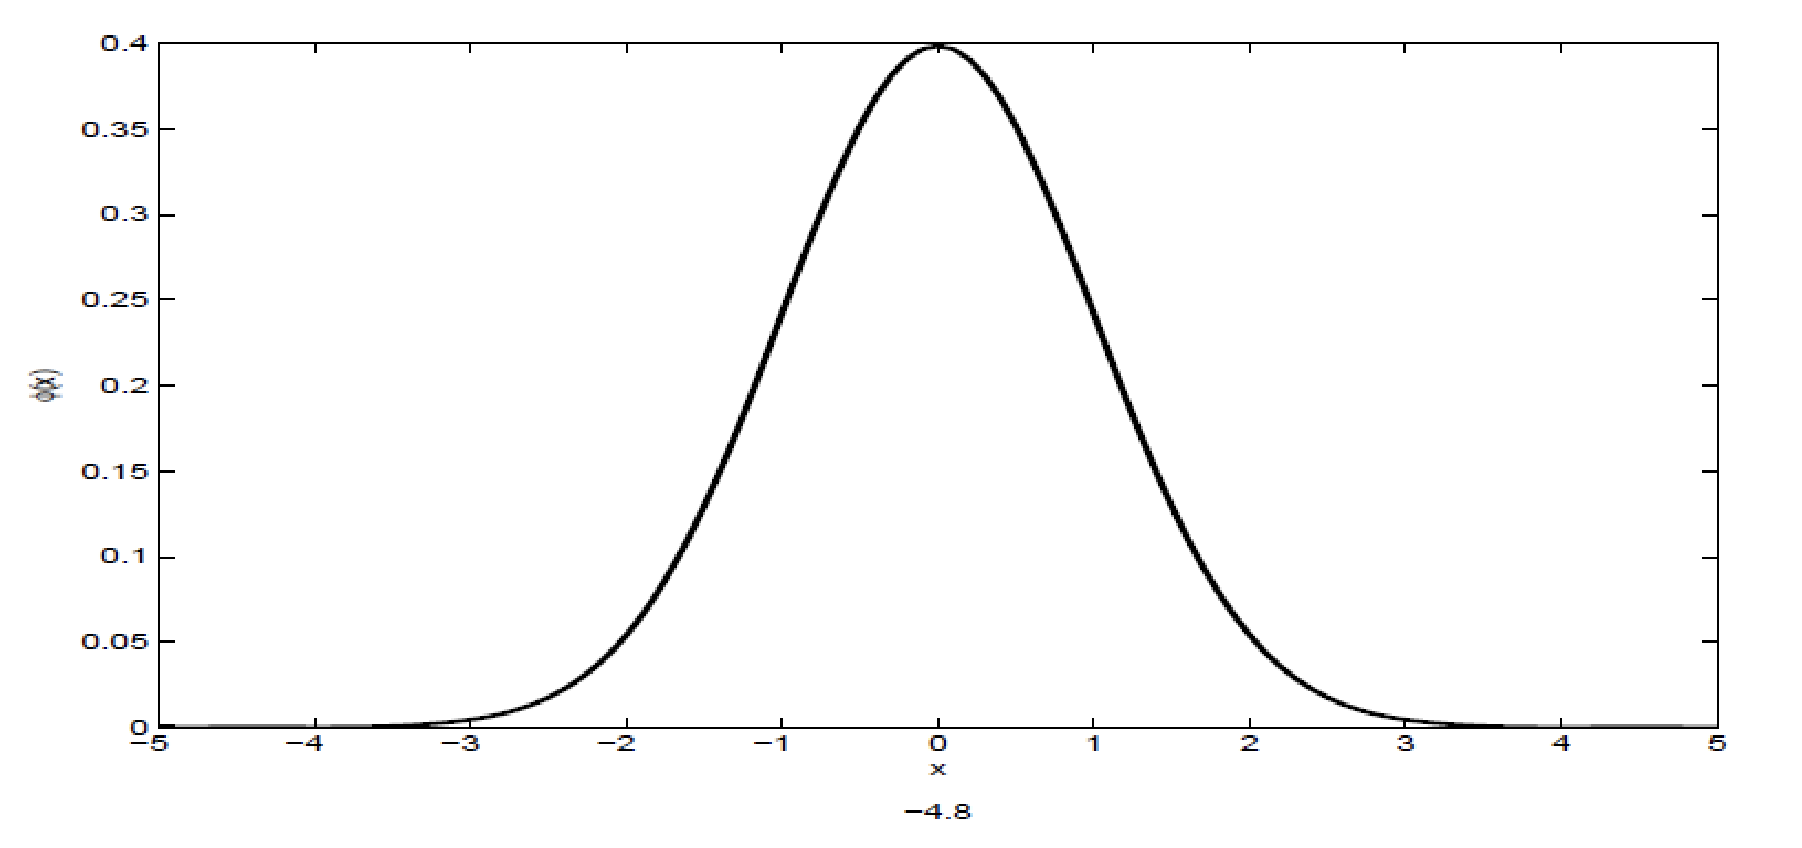
\includegraphics[width=1.05\linewidth]{img/standard-normal.png}
      \caption{The Standard Normal $N(0,1)$ p.d.f.}
    \end{minipage}\hfill
    \begin{minipage}{0.48\textwidth}
      \centering
      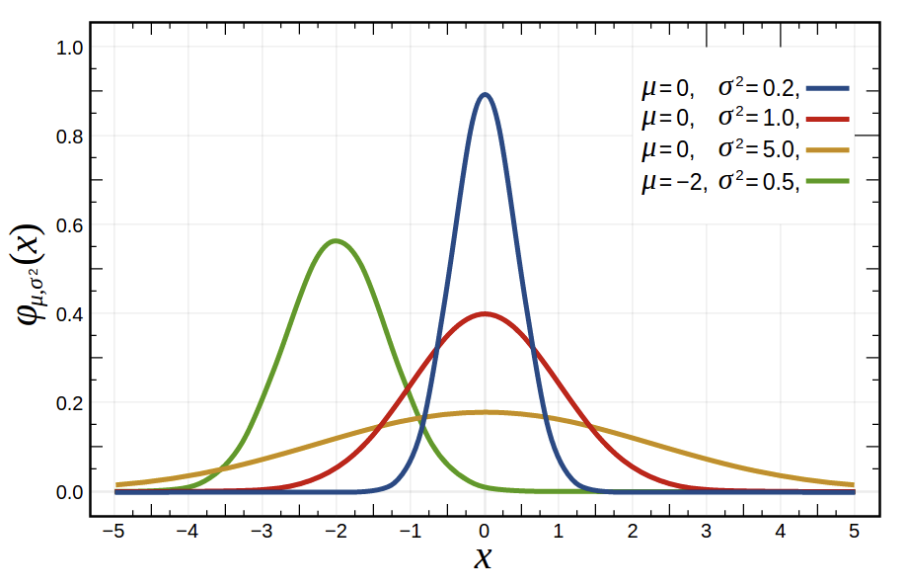
\includegraphics[width=0.9\linewidth]{img/different-normal.png}
      \caption{Some p.d.f.s}
    \end{minipage}
 \end{figure}

 \begin{note}
    For the first figure, we have $\mu = 0$ and $\sigma^2 = 1$. Normal distributions are symmetric about the mean (the line $x = \mu$), so 50\% on each side.
 \end{note}

 \vspace{3mm}

\textbf{Effects of the Mean and the Variance}

\begin{figure}[!htb]
    \begin{minipage}{0.48\textwidth}
      \centering
      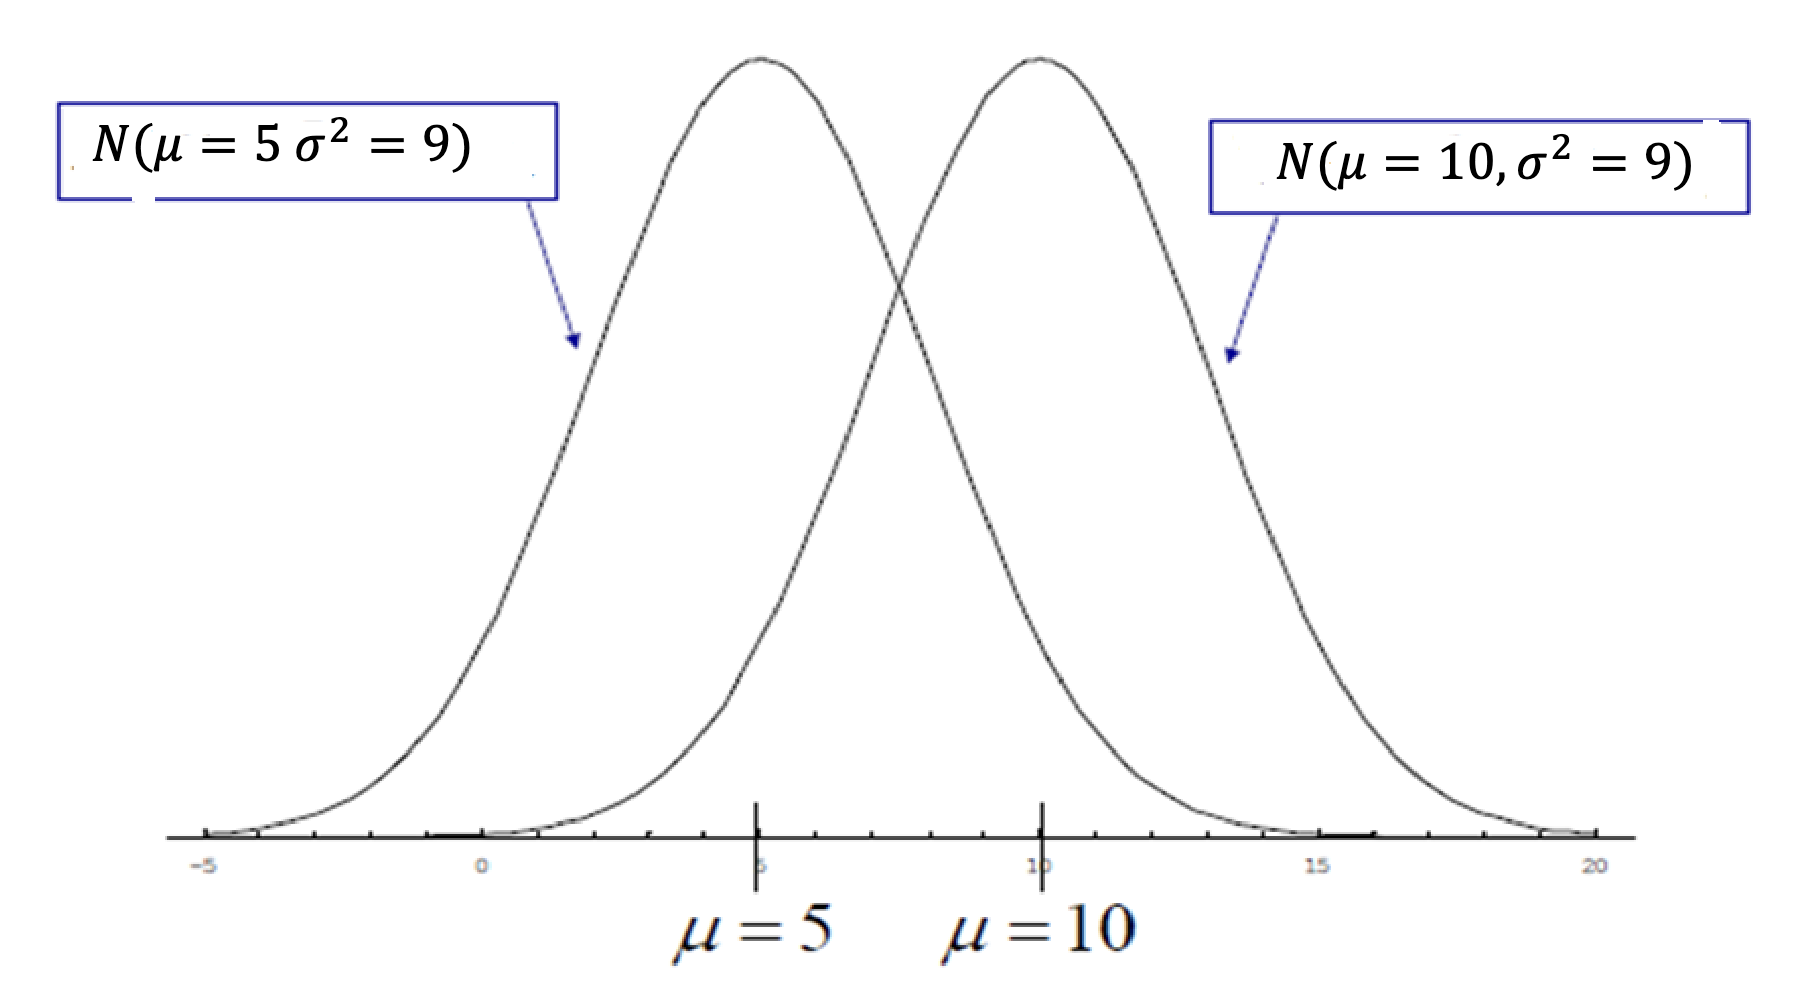
\includegraphics[width=1\linewidth, height=0.2\textheight]{img/effect-of-mean.png}
      \caption{Effect of $\mu$.}
    \end{minipage}\hfill
    \begin{minipage}{0.48\textwidth}
      \centering
      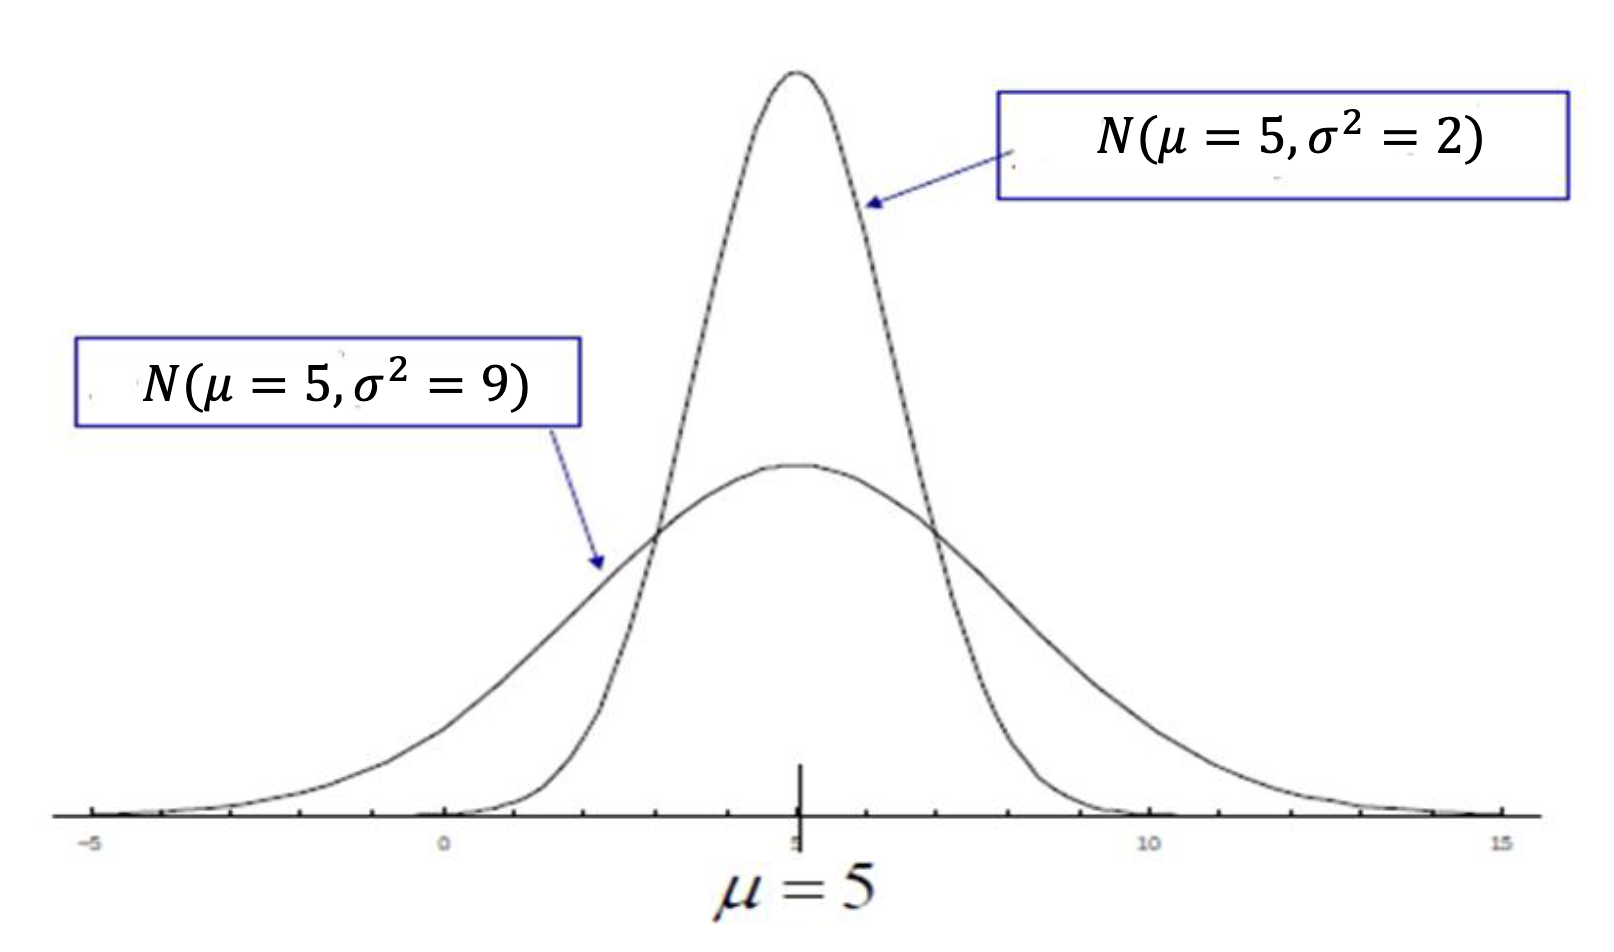
\includegraphics[width=1\linewidth]{img/effect-of-var.png}
      \caption{Effect of $\sigma^2$.}
    \end{minipage}
 \end{figure}

 \pagebreak

 \begin{note}
    \phantom{}\
    \begin{itemize}
        \item The mean shifts the distribution horizontally (shifts to the right as $\mu$ increases).
        \item The variance stretches the distribution (gets thicker and lower as $\sigma^2$ increases). 
    \end{itemize}
 \end{note}

 \begin{example}
    Heights or weights of males (or females) in large populations tend to follow a Normal distribution.
 \end{example}

 \textbf{The C.D.F.} of $N(\mu,\sigma^2)$ is
 \[
    F(x) = \int_{-\infty}^{x} \frac{1}{\sqrt{2\pi\sigma}} e^{-\frac{1}{2}\left(\frac{y-\mu}{\sigma}\right)^2} \, dy \quad x \in \R.
\]

\begin{note}
    Numerical methods are used to compute its value. 
\end{note}

$N(0,1)$ is called the ``\textbf{standard}'' Normal distribution with $\mu = 0$ and $\sigma = 1$. We have a ``new'' random variable $Z = \dis \frac{X - \mu}{\sigma}$, which is distributed as $Z \sim \text{N}(0,1)$.

\begin{theorem}
    Let $X \sim \text{N}(\mu,\sigma^2)$ and defined $Z = \dis \frac{X - \mu}{\sigma}$. Then $Z \sim \text{N}(0,1)$ and
    \[
        P(X \leq x) = P \left( Z \leq \frac{X - \mu}{\sigma} \right).
    \]
\end{theorem}

\begin{note}
    If we can compute the c.d.f. for $N(0,1)$, then we can compute it for other $N(\mu,\sigma^2)$ as well.
\end{note}

\textbf{What is this transformation doing?}

Consider the distribution of heights of young women aged 18 to 24. The distribution is approximately Normal with mean 64.5 inches and standard deviation 2.5 inches. We have $X \sim \text{N}(64.5,2.5^2)$.

\begin{figure}[htbp]
    \center
    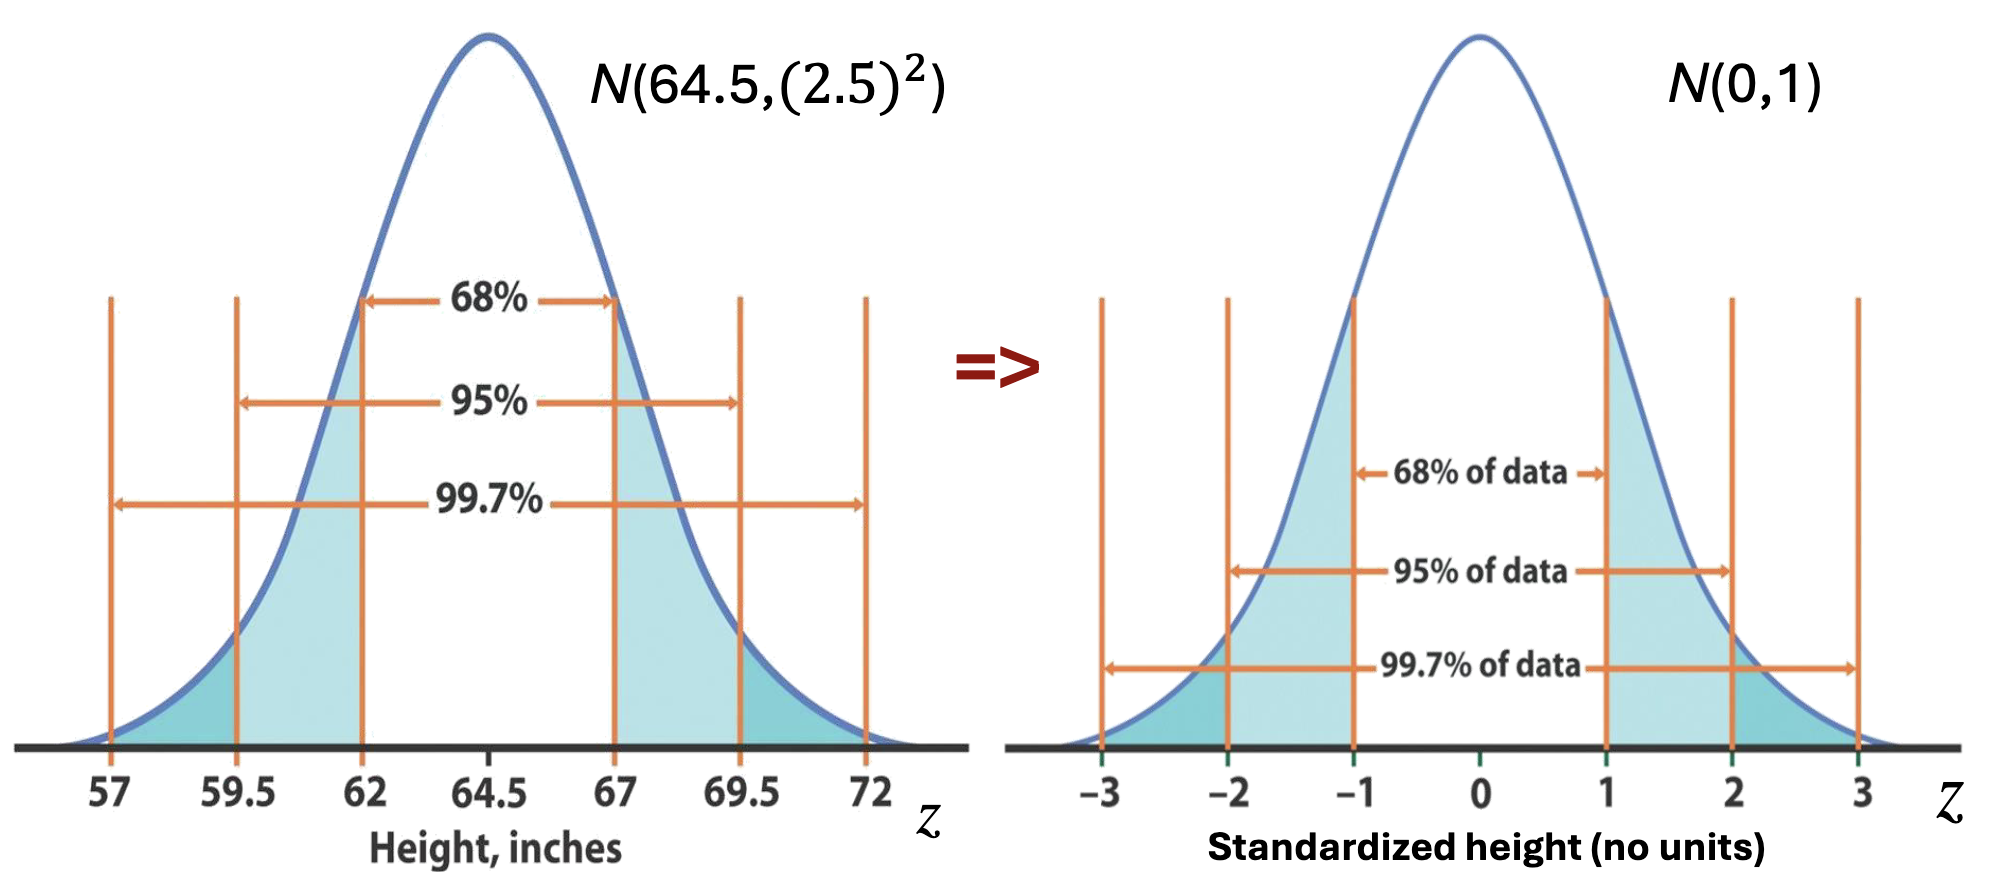
\includegraphics[scale=0.3]{img/Z-distribution.png}
    \caption{Transform to the standard Normal distribution.}
\end{figure}

\begin{theorem}[\textbf{Other Properties of Normal Distribution}]
    \phantom{}\\
    If $X \sim \text{N}(\mu,\sigma^2)$, then we have
    \begin{itemize}
        \item Symmetric about the mean: \vspace{-3mm}
        \[
            P(X \leq \mu - t) = P(X \geq \mu + t)
        \]
        or
        \[
            P(X \leq \mu + t) = P(X \geq \mu - t).
        \]
        \item Density is unimodal: peak is at $\mu$. Furthermore, mean and median also at $x = \mu$.
    \end{itemize}
\end{theorem}

\begin{figure}[htbp]
    \center
    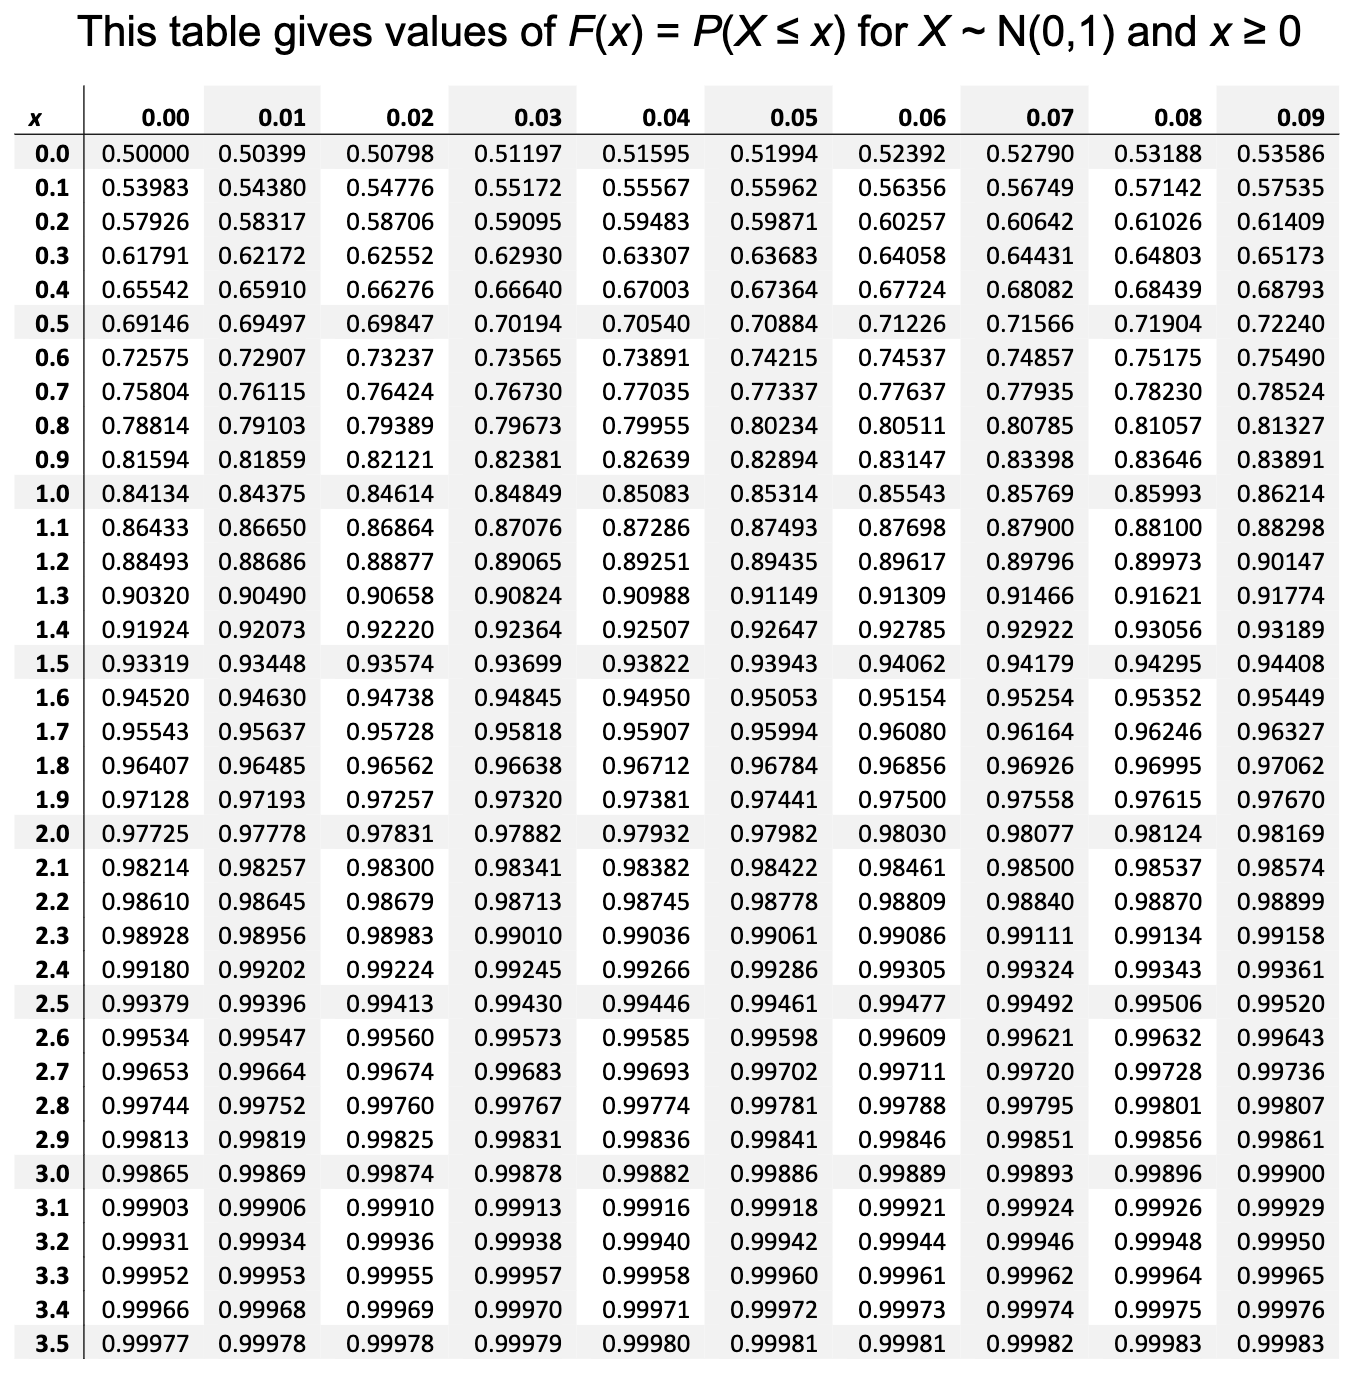
\includegraphics[scale=0.55]{img/N-CDF-table.png}
    \caption{Standard Normal Distribution c.d.f. values.}
\end{figure}

\textbf{How do we use the c.d.f. table?}

\begin{figure}[htbp]
    \center
    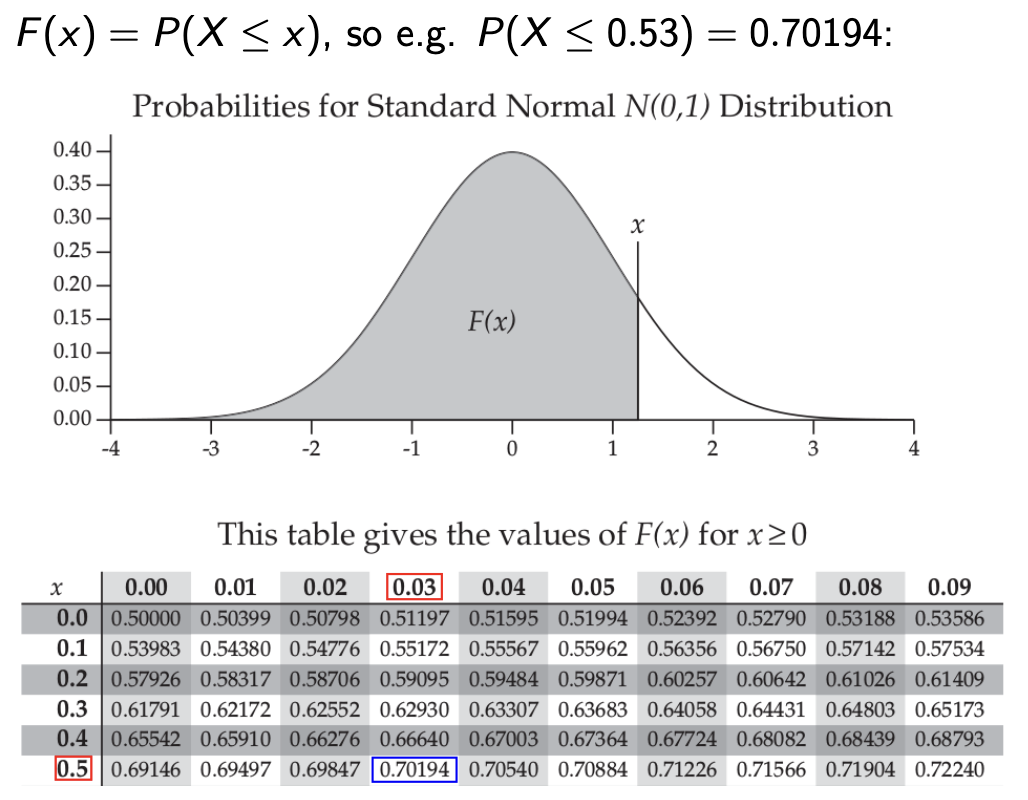
\includegraphics[scale=0.6]{img/N-table-example.png}
    \caption{Example of using the c.d.f. table.}
\end{figure}


\begin{example}
    Find a number $b$ such that $P(|Z| \leq b) = 0.95$. 

    \textbf{Solution:} Note that $P(|Z| \leq b) = P(-b \leq Z \leq b) = 0.95$. By symmetry, the probability outside $(-b,b)$ must be 0.05.

    $\implies P(Z \leq -b) + P(Z \geq b) = 0.05$. Furthermore, $P(Z \leq -b) = P(Z \geq b) = 0.025$ by symmetry again.

    $\implies P(Z \leq b) = 0.025 + 0.95 = 0.975.$ Looking for the value in the table, we get $b = 1.96$.
\end{example}

\begin{remark}
    Drawing out the normal distribution helps a lot!!!!! \\
\end{remark}

\textbf{Gaussian Distribution:} Another name for the Normal distribution. $X \sim \text{G}(\mu, \sigma)$ means that $X$ has  Gaussian distribution with mean $\mu$ and standard deviation $\sigma$. 

\begin{example}
    We can write $X \sim \text{N}(1,4)$ as $X \sim \text{G}(1,2)$.
\end{example}

\pagebreak

\begin{theorem}[\textbf{Standardization}]
    \[
        P(X \leq x) = P(\frac{X - \mu}{\sigma} \leq \frac{x - \mu}{\sigma}) = P(Z \leq \frac{x - \mu}{\sigma}),
    \]
    where $Z \sim \text{N}(0,1)$.
\end{theorem}

\begin{remark}
    Standardization can also be used for calculating other types of probabilities:
    \begin{itemize}
        \item $P(X > x) = P(Z > \frac{x - \mu}{\sigma})$.
        \item $P(a < X < b) = P(\frac{a - \mu}{\sigma} < Z < \frac{b - \mu}{\sigma}) = P(Z < \frac{b - \mu}{\sigma}) - P(Z < \frac{a - \mu}{\sigma})$. \\
    \end{itemize}
\end{remark}

\begin{example}
    Suppose $X \sim \text{N}(10,2)$, find $P(|X-10| \leq 3)$.

    \textbf{Solution:} 
    \begin{align*}
        P(|X-10| \leq 3) &= P(-3 \leq X - 10 \leq 3) \\
        &= P(7 \leq X \leq 13) \\
        &= P(\frac{7 - 10}{\sqrt{2}} \leq \frac{X - \mu}{\sigma} \leq \frac{13 - 10}{\sqrt{2}}) \quad \text{(standardize)} \\
        &= P(-2.12 \leq Z \leq 2.12) \\
        &= P(Z \leq 2.12) - P(Z \leq -2.12) \\
        &= P(Z \leq 2.12) - P(Z \geq 2.12) \\
        &= P(Z \leq 2.12) - \left[ 1 - P(Z \leq 2.12) \right] \\
        &= 2P(Z \leq 2.12) - 1 \\
        &= (2 \times 0.983) - 1 = 0.966.
    \end{align*}
\end{example}

\begin{example}[\textbf{Exercise}]
    Suppose $X \sim \text{N}(-7,14)$, find $P(|X+7| \geq 8)$. \\
    \textbf{Ans: $2 - 2P(Z \leq 2.14) = 0.03236$}.
\end{example}

\pagebreak

\begin{example}
    Suppose a certain mechanical component produced by a company has a width that is normally distributed with a mean $\mu = 2600$ and a standard deviation $\sigma = 0.6$.
    \begin{enumerate}[label=(\alph*)]
        \item What proportion of the components have a width outside the range 2599 to 2601?
        \item If the company needs to be able to guarantee to its purchaser that no more than 1 in 1000 of the
        components have a width outside the range 2599 to 2601, by how much does the value of $\sigma$ need to be reduced?
    \end{enumerate}

    \textbf{Solution:} 
    \begin{enumerate}[label=(\alph*)]
        \item Let $X = $ the width of a component. Then $X \sim \text{N}(2600,0.6^2)$. \vspace{-2mm}
        \begin{align*}
            P(X > 2601) + P(X < 2599) &= P(Z > \frac{2601 - 2600}{0.6}) + P(Z < \frac{2599 - 2600}{0.6}) \\
            &= P(Z > 1.67) + P(Z < -1.67) \quad \text{(standardize)} \\
            &= \left[ 1 - P(Z \leq 1.67) \right] + \left[ 1 - P(Z \leq 1.67) \right] \\
            &= 2 - 2P(Z \leq 1.67) \\
            &= 2 - (2 \times 0.95254) = 0.095.
        \end{align*}
        \item \phantom{} \vspace{-2mm}
        \begin{align*}
            P(X > 2601) + P(X < 2699) &\leq 0.001 \\
            1 - P(2599 < X < 2601) &\leq 0.001 \\
            P(2599 < X < 2601) &\geq 0.999 \\
            P(\frac{2599-2600}{\sigma} < Z < \frac{2601 - 2600}{\sigma}) &\geq 0.999 \\
            P(-\frac{1}{\sigma} < Z < \frac{1}{\sigma}) &\geq 0.999
        \end{align*}
        Using a sketch of the normal distribution, the probability within $(-\frac{1}{\sigma},\frac{1}{\sigma})$ $\geq$ 0.999. This means that we have probability $\leq$ 0.0005 at each side of the distribution. \\
        $\implies P(Z \leq \frac{1}{\sigma}) \geq 0.9995$ So, $\frac{1}{\sigma} = 3.29$.

        Therefore, we must have $\sigma \leq 0.30395$, need to reduce $\sigma$ by about 0.29605.
    \end{enumerate}
\end{example}

\pagebreak

\begin{figure}[htbp]
    \center
    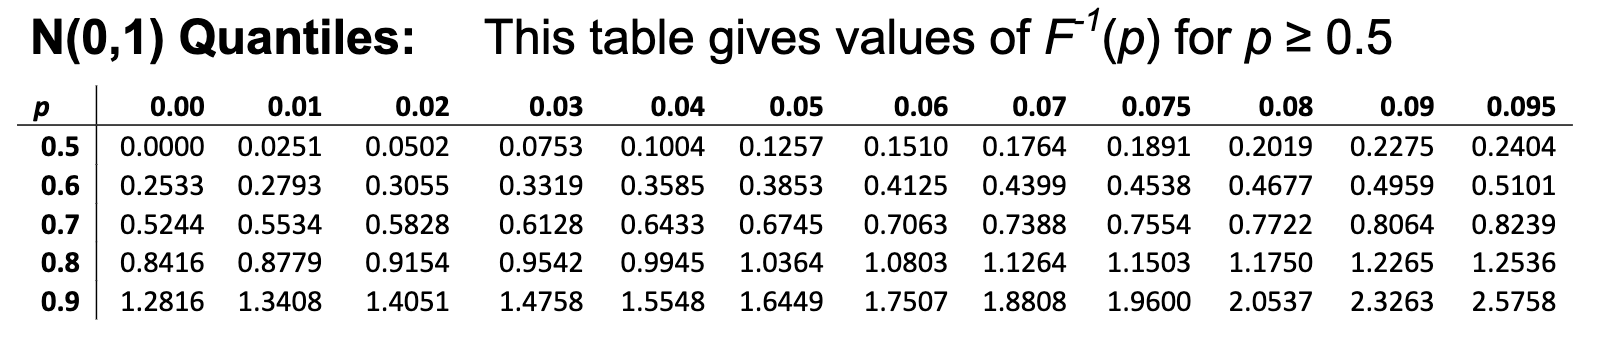
\includegraphics[scale=0.55]{img/quantiles-normal.png}
    \caption{Standard Normal Distribution Quantiles.}
\end{figure}

\begin{example}
    Let $X \sim \text{N}(0.28,0.05^2)$. Find the 90th quantile.

    \textbf{Solution:} $F^{-1}(0.9) = 1.2816 = Z$. Since $\dis Z = \frac{X-0.28}{0.05}$, we have $X = 0.344$. 
\end{example}

\newpage